\pdfminorversion=4
\documentclass[]{beamer}
\mode<presentation>
% Time-stamp: <2021-07-10 16:35:01 (jonahm)>

% beamer stuff
% Gives us the bottom line with all the goodies
\useoutertheme{infolines}
% Just the theme to use. Should be built into bemaer. Setting the
% height gets rid of a whole lot of whitespace
\usetheme[height=7mm]{Rochester}
\usefonttheme{serif}
% Usually beamer gives you navigation hyperlinks on the bottom
% right. I turned this off. It's annoying.
\setbeamertemplate{navigation symbols}{} 
% Makes my text boxes look pretty
\setbeamertemplate{blocks}[rounded][shadow=true] 
% Makes my bullet points 3d balls
\setbeamertemplate{items}[ball]

% Josh's packages
\usepackage{multimedia}
\usepackage{graphicx}

% Packages for me
\usepackage{amsmath,amssymb,latexsym,amsthm}
\usepackage[mathscr]{eucal}
\usepackage{mathrsfs}
\usepackage{verbatim}
\usepackage{braket}
\usepackage{listings}
\usepackage{xcolor}
% \usepackage[usenames,dvipsnames,svgnames,table]{xcolor}
\usepackage{fancybox}
\usepackage{animate}
% \usepackage{media9}
\usepackage{multicol}
\usepackage{mdframed}
\usepackage{hyperref}
%\usepackage{scalerel}
\usepackage[outline]{contour}
\contourlength{1.2pt}

% Macros

%Blackboard Bold
\newcommand{\R}{\mathbb{R}}
\newcommand{\Z}{\mathbb{Z}}
\newcommand{\N}{\mathbb{N}}
\newcommand{\Q}{\mathbb{Q}}
\newcommand{\A}{\mathbb{A}}
\newcommand{\E}{\mathbb{E}}
% other
\newcommand{\eval}{\biggr\rvert} %evaluated at
\newcommand{\myvec}[1]{\mathbf{#1}} % vectors for me
% total derivatives 
\newcommand{\diff}[2]{\frac{d #1}{d #2}} 
\newcommand{\dd}[1]{\frac{d}{d #1}}
% partial derivatives
\newcommand{\pd}[2]{\frac{\partial #1}{\partial #2}} 
\newcommand{\pdd}[1]{\frac{\partial}{\partial #1}} 
% Order operator
\DeclareRobustCommand{\orderof}{\ensuremath{\mathcal{O}}}

% braces
\newcommand{\paren}[1]{\left( #1 \right)}
\newcommand{\sqrbrace}[1]{\left[ #1 \right]}
\newcommand{\curlybrace}[1]{\left\{ #1 \right\}}
\newcommand{\inner}[1]{\paren{#1}}
\newcommand{\norm}[1]{\left| #1 \right|_2}

% g
\newcommand{\detg}{\sqrt{-g}}

% neutrinos
\newcommand{\eepsilon}{\epsilon} % energy
\newcommand{\fin}{f\in \{\nu_e,\nu_{\bar{e}},\nu_x\}}
\newcommand{\sign}{\text{sign}(f)}
\newcommand{\jnuf}{j_{\eepsilon,f}}
\newcommand{\etanuf}{\eta_{\eepsilon,f}}
\newcommand{\Inuf}{I_{\eepsilon,f}}
\newcommand{\chinuf}{\chi_{\eepsilon,f}}
\newcommand{\sigmanuf}{\sigma_{\eepsilon,f}}
\newcommand{\alphanuf}{\alpha_{\eepsilon,f}}
\newcommand{\numin}{\nu_{\text{min}}}
\newcommand{\numax}{\nu_{\text{max}}}


% tikz
\usepackage{tikz}
\usepackage{pgfplots}
\usetikzlibrary{arrows}
\usetikzlibrary{decorations.pathmorphing}
\usetikzlibrary{decorations.markings}
\usetikzlibrary{arrows.meta,bending}

% Keys to support piece-wise uncovering of elements in TikZ pictures:
% \node[visible on=<2->](foo){Foo}
% \node[visible on=<{2,4}>](bar){Bar}   % put braces around comma expressions
% 
% Internally works by setting opacity=0 when invisible, which has the 
% adavantage (compared to \node<2->(foo){Foo} that the node is always there, hence
% always consumes space plus that coordinate (foo) is always available.
% 
% The actual command that implements the invisibility can be overriden
% by altering the style invisible. For instance \tikzsset{invisible/.style={opacity=0.2}}
% would dim the "invisible" parts. Alternatively, the color might be set to white, if the
% output driver does not support transparencies (e.g., PS) 
% 
\tikzset{
  invisible/.style={opacity=0},
  visible on/.style={alt={#1{}{invisible}}},
  alt/.code args={<#1>#2#3}{%
    \alt<#1>{\pgfkeysalso{#2}}{\pgfkeysalso{#3}} % \pgfkeysalso doesn't change the path
  },
}

% some nice flowchart features
\tikzset{
    mynode/.style={rectangle,rounded corners,draw=black, top color=white, bottom color=yellow!50,very thick, inner sep=1em, minimum size=3em, text centered},
    myarrow/.style={->, >=latex', shorten >=1pt, thick},
    mylabel/.style={text width=7em, text centered} 
}  

% squigly arrow
\tikzset{zigzag it/.style={decorate, decoration=zigzag}}

% Color morphing arrow
\tikzset{colormorph/.style n args={3}{
    postaction={
    decorate,
    decoration={
    markings,
    mark=between positions 0 and \pgfdecoratedpathlength step 0.5pt with {
    \pgfmathsetmacro\myval{multiply(
        divide(
        \pgfkeysvalueof{/pgf/decoration/mark info/distance from start}, \pgfdecoratedpathlength
        ),
        100
    )};
    \pgfsetfillcolor{#3!\myval!#2};
    \pgfpathcircle{\pgfpointorigin}{#1};
    \pgfusepath{fill};}
}}}}

% define a really nice visible "purple"
\definecolor{gimppurple}{HTML}{AD26FB}
% a light grey
\definecolor{lightgrey}{HTML}{E0E0E0}
% for highlighting
\definecolor{deepblue}{rgb}{0,0,0.5}
\definecolor{deepred}{rgb}{0.6,0,0}
\definecolor{deepgreen}{rgb}{0,0.5,0}

% fonts
% Default fixed font does not support bold face
\DeclareFixedFont{\ttb}{T1}{txtt}{bx}{n}{12} % for bold
\DeclareFixedFont{\ttm}{T1}{txtt}{m}{n}{12}  % for normal

% Python style for highlighting
\newcommand\pythonstyle{\lstset{
language=Python,
basicstyle=\ttm,
otherkeywords={self},
keywordstyle=\ttb\color{deepblue},
emph={__init__},           
emphstyle=\ttb\color{deepred},
commentstyle=\ttfamily\color{deepred},
stringstyle=\color{deepgreen},
frame=tb,                     
showstringspaces=false        
}}

% Python environment
\lstnewenvironment{python}[1][]
{
\pythonstyle
\lstset{#1}
}
{}

\newcommand{\backupbegin}{
   \newcounter{finalframe}
   \setcounter{finalframe}{\value{framenumber}}
}
\newcommand{\backupend}{
   \setcounter{framenumber}{\value{finalframe}}
}

% Automatically generates section breaker slides
\AtBeginSection[]{
  \begin{frame}[plain]
  \vfill
  \centering
  \begin{beamercolorbox}[sep=8pt,center,shadow=true,rounded=true]{title}
    \usebeamerfont{title}\insertsectionhead\par%
  \end{beamercolorbox}
  \vfill
  \end{frame}
}

\title[DR Review]{Neutrino Transport for Compact Objects}
% \subtitle{Models and Implications}
\author[J. Miller]{\textcolor{blue}{Jonah M. Miller},\\
  T. Sprouse, S. Curtis, S. De,\\
  Many More...}
\institute[LANL]{Los Alamos National Laboratory}
% \titlegraphic{\vspace{1cm}}
% \titlegraphic{\includegraphics[height=0.25\textheight]{3d_render}}
\date[7/14/21]{TCAN Workshop}

\graphicspath{{figures/}}

\begin{document}

\begin{frame}[plain]
    \tikz [remember picture, overlay] 
    \node at ([xshift=2cm,yshift=-2cm]current page.west)
    {\includegraphics[width=0.25\textwidth,clip,trim={150 0 150 0}]{3d_render}};
    \tikz [remember picture, overlay] 
    \node at ([xshift=-2cm,yshift=-2cm]current page.east)
    {\includegraphics[width=0.25\textwidth,clip,trim={0 0 0 0}]{visit0006-gimp3}};
  \titlepage
\end{frame}

\begin{frame}
  \frametitle{When is Neutrino Transport Relevant?}
  \begin{itemize}
  \item Focus here on disks, more is relevant:
    \begin{itemize}
    \item in-spiral+merger
    \item core-collapse+bounce
    \end{itemize}
  \end{itemize}
  \begin{columns}
    \begin{column}{6cm}
      \resizebox{\columnwidth}{!}{
          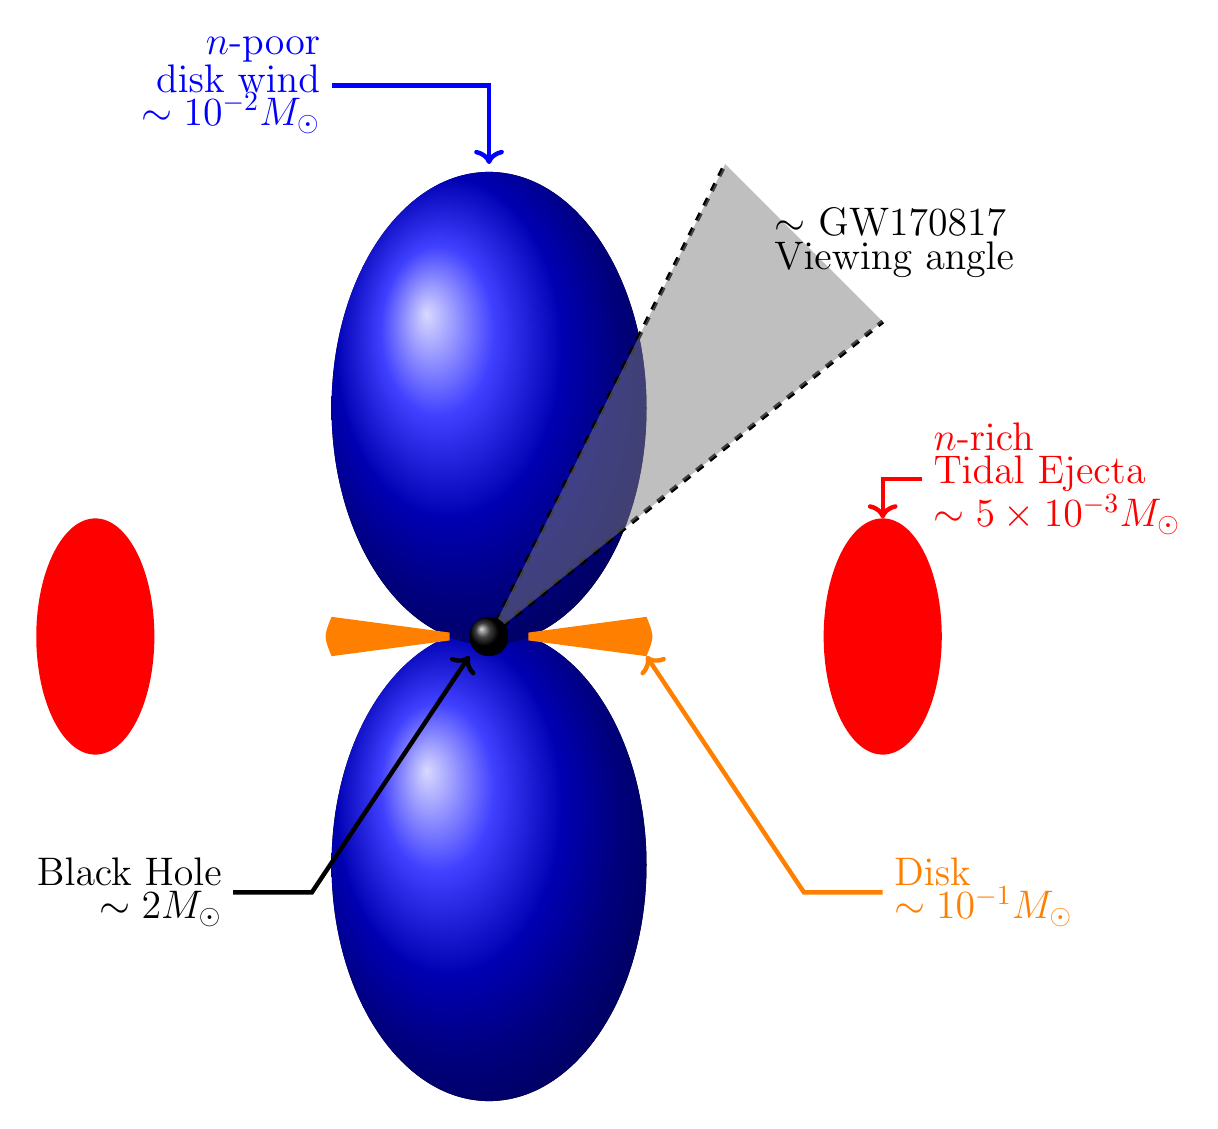
\begin{tikzpicture}
            \coordinate (origin) at (0,0);
            \pgfmathsetmacro{\dbx}{0.5}
            \pgfmathsetmacro{\dby}{0.05}
            \pgfmathsetmacro{\dex}{2.}
            \pgfmathsetmacro{\dey}{0.25}
            \pgfmathsetmacro{\dcc}{2.1}
            \pgfmathsetmacro{\tcx}{5.0}

            \foreach \i in {-1,1}
            {
              \fill[ball color=blue] (0, \i*2.9) ellipse (2 and 3);
            }

            \foreach \i in {-1,1}
            {
              % disk
              \fill[color=orange]
              (\i*\dbx,\dby) -- (\i*\dex,\dey)
              .. controls (\i*\dcc,0) .. (\i*\dex,-\dey)
              -- (\i*\dbx,-\dby) -- cycle;

              % tidal ejecta
              \fill[color=red] (\i*\tcx,0) ellipse (0.75 and 1.5);
            }

            % viewing
            \draw[dashed,ultra thick,black] (origin) -- (5,4);
            \draw[dashed,ultra thick,black] (origin) -- (3,6);
            \fill[color=gray,opacity=0.5] (origin) -- (5,4) -- (3,6) -- cycle;
            \node[right,align=left] at (3.5,5)
            {\Large $\sim$ GW170817\\ \Large Viewing angle};

            % bh
            \shade[ball color=black] (origin) circle (0.25);

            % text
            \draw[<-,red, ultra thick] (\tcx,1.5)
            -- ++(0.,0.5) -- ++(0.5,0)
            node[right,align=left]
            {\Large \color{red}$n$-rich\\\Large Tidal Ejecta\\ \Large $\sim 5\times 10^{-3}M_{\odot}$};

            \draw[<-,blue, ultra thick] (0,6) -- ++(0,1) -- ++(-2,0)
            node[left,align=right]
            {\Large \color{blue}$n$-poor\\\Large disk wind\\\Large $\sim 10^{-2}M_{\odot}$};

            \draw[<-,orange, ultra thick] (\dex,-\dey)
            -- ++(2,-3) -- ++(1,0)
            node[right,align=left]
            {\Large \color{orange}Disk\\\Large $\sim 10^{-1}M_{\odot}$};

            \draw[<-,black, ultra thick] (-0.25,-0.25)
            -- ++(-2,-3) -- ++(-1,0)
            node[left,align=right]
            {\Large \color{black}Black Hole\\ \Large $\sim 2 M_{\odot}$};
          \end{tikzpicture}
        }
    \end{column}
    \begin{column}{6cm}
      \resizebox{\columnwidth}{!}{
        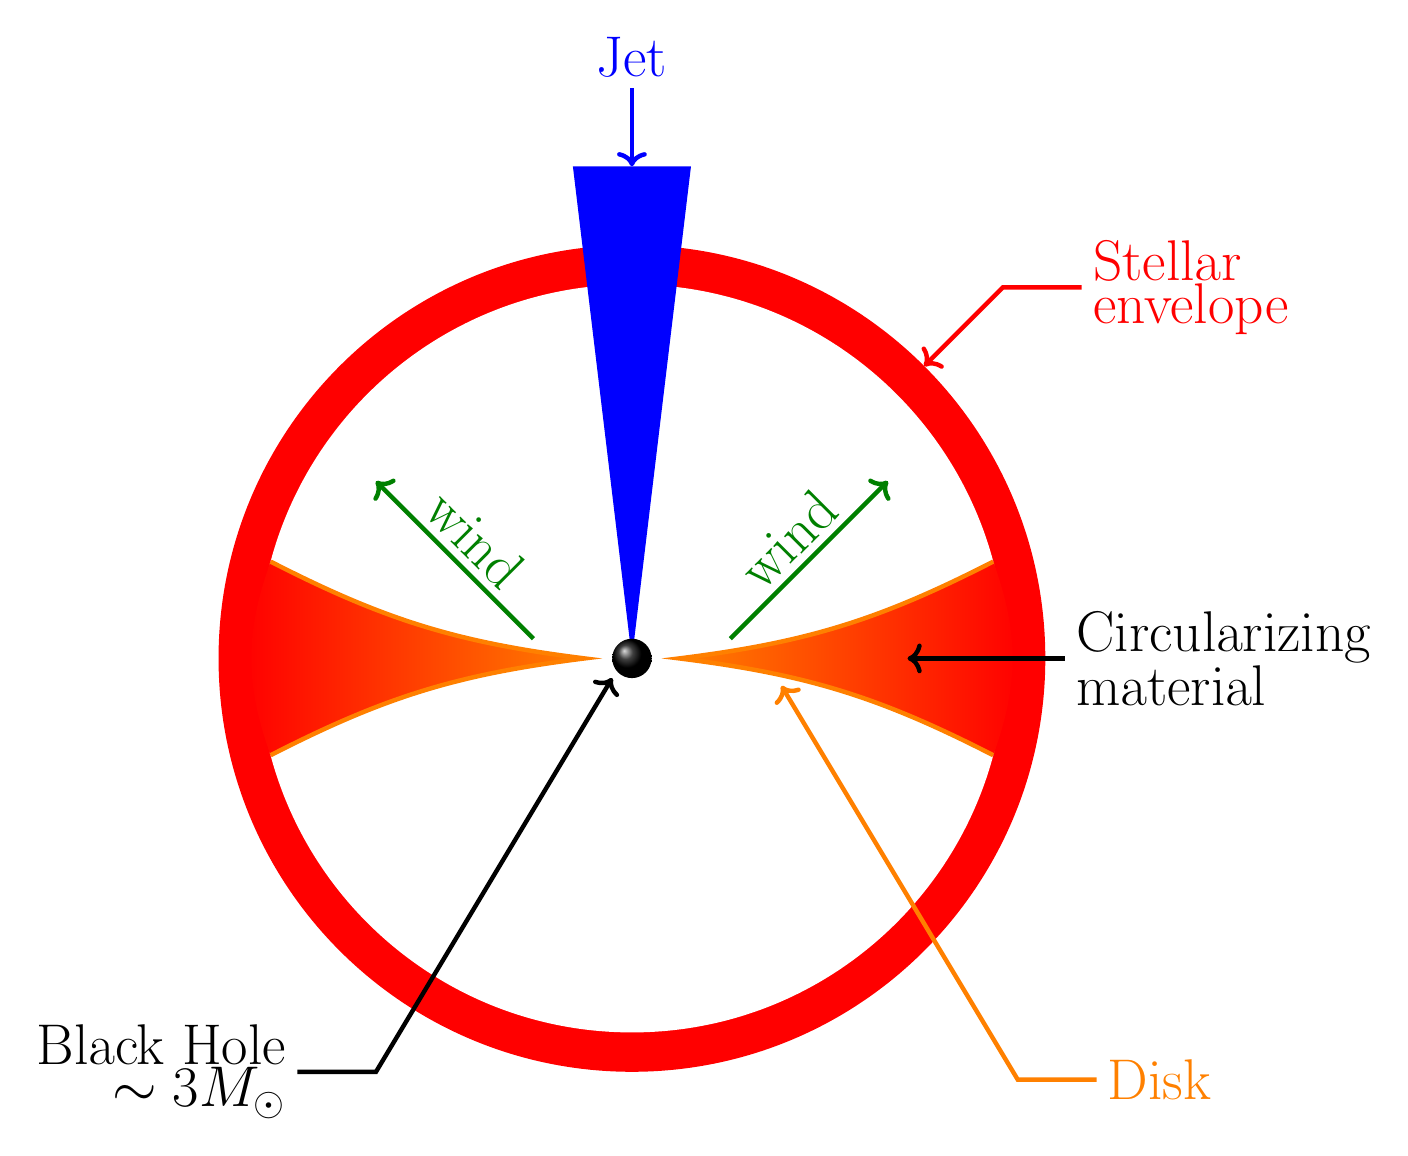
\begin{tikzpicture}
          \coordinate (origin) at (0,0);
          \pgfmathsetmacro{\pi}{3.14159}
          \pgfmathsetmacro{\dbx}{0.5}
          \pgfmathsetmacro{\dby}{0.05}
          \pgfmathsetmacro{\dex}{2.}
          \pgfmathsetmacro{\dey}{0.25}
          \pgfmathsetmacro{\dcc}{2.1}
          \pgfmathsetmacro{\tcx}{5.0}
          \pgfmathsetmacro{\rstar}{5}
          \pgfmathsetmacro{\wstar}{0.25}
          \pgfmathsetmacro{\wjet}{0.75}
          \pgfmathsetmacro{\tangle}{{45}}
          \pgfmathsetmacro{\tsx}{{(\rstar+\wstar)*cos(\tangle)}}
          \pgfmathsetmacro{\tsy}{{(\rstar+\wstar)*sin(\tangle)}}

          \pgfmathsetmacro{\cangle}{15}
          \pgfmathsetmacro{\cx}{(\rstar-\wstar)*cos(\cangle)}
          \pgfmathsetmacro{\cy}{(\rstar-\wstar)*sin(\cangle)}
          % \pgfmathsetmacro{\cend}{\dex + 0.1}
          \pgfmathsetmacro{\cend}{\dbx + 0.1}

          \newcommand{\msize}{\huge}

          % star
          \fill [color=red] (origin) circle (\rstar+\wstar);
          \fill [color=white] (origin) circle (\rstar-\wstar);

          % circularization
          \fill[color=red,
          left color=orange,
          middle color=orange,
          right color=red]
          (\cx,\cy) to [bend left=10] (\cend,0)
          to [bend left=10] (\cx,-\cy)
          to [bend right=20] cycle;
          
          \draw[orange,ultra thick]
          (\cx,\cy) to [bend left=10] (\cend, 0)
          to [bend left=10] (\cx,-\cy);

          \fill[color=red,
          right color=orange,
          middle color=orange,
          left color=red]
          (-\cx,\cy) to [bend right=10] (-\cend,0)
          to [bend right=10] (-\cx,-\cy)
          to [bend left=20] cycle;
          
          \draw[orange,ultra thick]
          (-\cx,\cy) to [bend right=10] (-\cend, 0)
          to [bend right=10] (-\cx,-\cy);

          % \foreach \i in {-1,1}
          % {
          %   % disk
          %   \fill[color=orange]
          %   (\i*\dbx,\dby) -- (\i*\dex,\dey)
          %   .. controls (\i*\dcc,0) .. (\i*\dex,-\dey)
          %   -- (\i*\dbx,-\dby) -- cycle;
          % }
          
          % jet
          \fill[color=blue] (origin) -- (-\wjet,1.25*\rstar) -- ++(2*\wjet,0) -- cycle;

          % bh
          \shade[ball color=black] (origin) circle (0.25);

          % wind
          \draw[deepgreen,ultra thick, ->]
          ({0.5*(\dbx + \dex)},\dey) -- ++(2,2);
          \draw ({0.5*(\dbx + \dex) + 1},{(\dey+1)})
          node[above,align=center,rotate=45]
          {\color{deepgreen}\msize wind};
          \draw[deepgreen,ultra thick, ->]
          ({-0.5*(\dbx + \dex)},\dey) -- ++(-2,2);
          \draw ({-(0.5*(\dbx + \dex) + 1)},{(\dey+1)})
          node[above,align=center,rotate=-45]
          {\color{deepgreen}\msize wind};          

          % text
          \draw[<-,orange, ultra thick] (\dex-0.1,-\dey-0.1)
          -- ++(3,-5) -- ++(1,0)
          node[right,align=left]
          {\msize \color{orange}Disk};
          
          \draw[<-,black, ultra thick] (-0.25,-0.25)
          -- ++(-3,-5) -- ++(-1,0)
          node[left,align=right]
          {\msize \color{black}Black Hole\\ \msize $\sim 3 M_{\odot}$};
          
          \draw[<-,red,ultra thick] (\tsx,\tsy)
          -- ++(1,1) -- ++(1,0)
          node[right,align=left]
          {\msize \color{red} Stellar\\ \msize envelope};

          \draw[<-,blue,ultra thick] (0, 1.25*\rstar) -- ++(0,1)
          node[above,align=center] {\msize \color{blue} Jet};

          \draw[<-,black,ultra thick]
          ({0.5*(\dex+\rstar)},0) -- ++(2,0) node[right,align=left]
          {\msize Circularizing\\ \msize material};
          
          \let\msize\undefined
        \end{tikzpicture}
      }
    \end{column}
  \end{columns}
\end{frame}

\begin{frame}
  \frametitle{Neutrino Transport Matters!}
  \begin{center}
    \includegraphics[height=0.8\textheight]{leptoneq/frame_0001}
    % \animategraphics[height=0.8\textheight,every=5,autoplay,loop,controls]
    % {5}{leptoneq/frame_}{0001}{0101}
  \end{center}
  \begin{tiny}
    \textbf{JMM}, B. R. Ryan, J. C. Dolence. ApJS \textbf{241} 30 (2019) 
  \end{tiny}
\end{frame}

\begin{frame}
  \frametitle{Transport Limits}
  \begin{itemize}
  \item Characterized by optical depth $\tau$ s.t. $I_\nu = I_{\nu}(s_0) e^{-\tau (s_0, s)}$
    \begin{itemize}
    \item Effective ``scattering optical depth'' also matters
    \end{itemize}
  \end{itemize}
  \vspace{1cm}
  \resizebox{12cm}{!}{
    \begin{tikzpicture}
      \draw[ultra thick, black, ->] (0,0) -- ++(8,0);
      % node[below] {$\tau$};

      \node[above,inner sep=0pt] at (0,0.25)
      {\includegraphics[height=1.5cm]{The_Sun_by_the_Atmospheric_Imaging_Assembly_of_NASA's_Solar_Dynamics_Observatory.jpg}};

      \node[above,inner sep=0pt] at (8,0.25)
      {\includegraphics[height=1.5cm]{ns-manhattan}};

      \node[above,inner sep=0pt] at (4,0.25)
      {\includegraphics[height=1.5cm]{disk_image_no_text}};

      \node[below,align=center] at (0,-0.25)
      {$\tau \ll 1$\\free-streaming};

      \node[below,align=center] at (8,-0.25)
      {$\tau \gg 1$\\diffusion};

      \node[below,align=center] at (4,-0.25)
      {Must solve\\full Boltzmann\\Equation};

    \end{tikzpicture}
  }
\end{frame}

\begin{frame}
  \frametitle{Transport Techniques}
  \begin{columns}
    \begin{column}{6cm}
      \begin{itemize}
      \item Full Boltzmann Solvers
        \begin{itemize}
        \item Mesh-based methods
          \begin{itemize}
          \item Discrete ordinates
          \item Sparse grids
          \item Spectral and finite differences
          \end{itemize}
        \item Mesh-free
          \begin{itemize}
          \item Monte Carlo
          \end{itemize}
        \end{itemize}
      \end{itemize}
    \end{column}
    \begin{column}{6cm}
      \begin{itemize}
      \item Approximate methods
        \begin{itemize}
        \item Cooling functions
        \item Leakage
        \item Flux-limited Diffusion
        \item Analytic moment closures
        \end{itemize}
      \item Hybrid methods
        \begin{itemize}
        \item Moment methods with flexible closures
        \item Diffusion + leakage, etc.
        \end{itemize}
      \end{itemize}
    \end{column}
  \end{columns}
\end{frame}

\begin{frame}
  \frametitle{Relevant Neutrino Interactions}
  \begin{tiny}
    \begin{tabular}{l | l | l }
    \hline
    \textbf{Type}&\textbf{Processes}&\textbf{Corrections/Approximations}\\
    \hline
    % \textbf{Emission}&&\\
    \hline
    Abs./Emis. on Neutrons & 
                             \begin{tabular}{@{}l@{}}
                               $\nu_e + n \leftrightarrow e^- + p$\\
                               $\nu_\mu + n \leftrightarrow \mu^- + p$
                             \end{tabular}
                 & 
                             \begin{tabular}{@{}l@{}}
                               Blocking/Stimulated
                               Abs.\\
                               Weak
                               Magnetism\\
                               Recoil
                             \end{tabular}\\
    \hline
    Abs./Emis. on Protons & 
                            \begin{tabular}{@{}l@{}}
                              $\bar{\nu}_e + p \leftrightarrow e^+ +
                              n$\\
                              $\bar{\nu}_\mu + p \leftrightarrow \mu^+
                              + n$\\
                            \end{tabular}
                 & 
                             \begin{tabular}{@{}l@{}}
                               Blocking/Stimulated
                               Abs.\\
                               Weak
                               Magnetism\\
                               Recoil
                             \end{tabular}\\
    \hline
    Abs./Emis. on Ions & $\nu_eA \leftrightarrow A'e^-$ & 
                                                                    \begin{tabular}{@{}l@{}}
                                                                      Blocking/Stimulated Abs.\\
                                                                      Recoil
                                                                    \end{tabular}\\
    \hline
    Electron Capture on Ions & $e^- + A \leftrightarrow A' + \nu_e$ &
                                                                                \begin{tabular}{@{}l@{}}
                                                                                  Blocking/Stimulated Abs.\\
                                                                                  Recoil
                                                                                \end{tabular}\\
                                                             
    \hline
    $e^+-e^-$ Annihilation & $e^+e^- \leftrightarrow \nu_i\bar{\nu}_i$&
                                                                    \begin{tabular}{@{}l@{}}
                                                                      single-$\nu$
                                                                      Blocking\\
                                                                      Recoil
                                                                    \end{tabular}\\
    \hline
    $n_i$-$n_i$ Brehmsstrahlung & $n_i^1 + n_i^2 \to n_i^3 +
                                      n_i^4 + \nu_i\bar{\nu}_i$ 
                                    & 
                                                \begin{tabular}{@{}l@{}}
                                                  single-$\nu$ Blocking\\
                                                  Recoil
                                                \end{tabular}\\
      \hline
      Proton scattering & $\nu_i + p \leftrightarrow \nu_i + p$
                                    & elastic/inelastic\\
      \hline
      Neutron scattering & $\nu_i + n \leftrightarrow \nu_i + n$
                                    & elastic/inealstic\\
      \hline
      Heavy ion scattering & $\nu_i + A \leftrightarrow \nu_i + A$
                                    &
                                      \begin{tabular}{@{}l@{}}
                                        ion-ion correlation\\
                                        electron polarization\\
                                        form-factor
                                      \end{tabular}\\
      \hline
    \end{tabular}
  \end{tiny}
  \begin{itemize}
  \item And this is ignoring Neutrino oscillations!
  \end{itemize}
  {\footnotesize Burrows, Reddy, Thompson, NPA \textbf{177}, 356, (2006)}
\end{frame}

\begin{frame}
  \frametitle{How Much Does Transport Matter for disks?}
  \begin{itemize}
  \item Interactions scaling/nucleon:
    \begin{itemize}
    \item $T^6$ typical in disks. Can be as sharp as $T^8$!
    \end{itemize}
  \end{itemize}
  \resizebox{12cm}{!}{
    \begin{tikzpicture}
      \coordinate (origin) at (0,0);

      \draw[blue] (origin) -- (5,3);

      \node[left] (tau1) at (0,2) {$\tau=1$};
      \draw[dashed,gray] (tau1) -- ++(5.5,0);

      \node[below] (m1) at (10./3.,0) {$10^0$};
      \draw[dashed,gray] (m1) -- ++(0,3.75)
      node[above] {\color{black}$10^{-1}$};
      
      \coordinate(tau2) at (0,1);
      \draw[dashed,gray] (tau2) -- ++(5,0);

      \node[below](m2) at (5./3.,0) {$10^{-1}$};
      \draw[dashed, gray] (m2) -- ++(0, 3.75)
      node[above] {\color{black}$10^{-2}$};

      \node[left] at (origin) {$\tau\ll 1$};
      \draw[ultra thick, black,->] (origin)
      -- ++(5, 0) node[below] {$\dot{M} (M_\odot/s)$};
      \draw[ultra thick, black, ->] (origin)
      -- ++(0, 3) node[left] {$\tau_\nu$};
      \draw[ultra thick, black, ->] (0,3.5)
      -- ++(5,0) node[above] {$M_d (M_\odot)$};

      \draw[<-,visible on=<1-2>] (5.2,3) -- ++(0.25,0) node[right,align=left]
      {\footnotesize \color{red}stay tuned};
      \node[inner sep=0pt,right, visible on=<3>] at (5,3) {\includegraphics[width=1cm]{curtis-pic}};
      \draw[<-,visible on=<1>] (5.2,2) -- ++(0.25,0) node[right,align=left]
      {\footnotesize abs. matters};
      \draw[<-,visible on=<2->] (5.2,2) -- ++(0.25,0) node[right,align=left]
      {\footnotesize $\sim 10^{-3}\dot{M}_{\text{ed}}$};

      \draw[<-] (5.2,1) -- ++(0.25,0) node[right,align=left]
      {\footnotesize emiss. doms.};

      \draw[<-] (0,-0.2) -- ++(0,-0.25) node[below,align=center]
      {\footnotesize no ignition};
    \end{tikzpicture}
    }
\end{frame}

\begin{frame}
  \frametitle{Ingredients In Neutrino Disk Modeling}
  \begin{itemize}
  \item General relativity
    \begin{itemize}
    \item Rotating black hole spacetime
    \end{itemize}
  \item Plasma physics
    \begin{itemize}
    \item Ideal magnetohydrodynamics
    \end{itemize}
  \item Nuclear physics
    \begin{itemize}
    \item Hot gas treated as being in nuclear-statistical equilibrium via \textbf{equation of state}
    \item Cooling outflow treated in postprocessing via \textbf{nuclear reaction networks}
    \end{itemize}
  \item Radiation physics
    \begin{itemize}
    \item Material is opaque to photons, can be incorporated in plasma physics
    \item Material \textit{not} opaque to \textbf{neutrinos}.
    \item Neutrinos can \textit{change the composition of the
        material} by converting neutrons to protons and vice versa.
    \end{itemize}
  \end{itemize}
\end{frame}

\begin{frame}
  \frametitle{Ingredients in Neutrino Disk Modeling}
  \begin{itemize}
  \item Mass conservation:
    \begin{small}
      \begin{displaymath}
        \partial_t \paren{{\color{red}\detg}\rho_0 u^t}
        + \partial_i\paren{{\color{red}\detg}\rho_0u^i} = 0
      \end{displaymath}
    \end{small}
  \item Momentum and Internal Energy Conservation:
    \begin{small}
      \begin{displaymath}
        \partial_t\sqrbrace{{\color{red}\detg} \paren{T^t_{\ \nu} + \rho_0u^t \delta^t_\nu}}
        + \partial_i\sqrbrace{{\color{red}\detg}\paren{T^i_{\ \nu} + \rho_0 u^i \delta^t_\nu}}
        = {\color{red}\detg} \paren{T^\kappa_{\ \lambda} {\color{red}\Gamma^\lambda_{\nu\kappa}} + {\color{blue}G_\nu}}
      \end{displaymath}
    \end{small}
  \item Magnetic Fields
    \begin{small}
      \begin{displaymath}
        \partial_t \paren{{\color{red}\detg} B^i}
        - \partial_j \sqrbrace{{\color{red}\detg}\paren{b^ju^i - b^i u^j}}
        = 0
      \end{displaymath}
    \end{small}
  \item Composition
    \begin{small}
      \begin{displaymath}
        \partial_t\paren{{\color{red}\detg}\rho_0 Y_e u^t}
        + \partial_i\paren{{\color{red}\detg}\rho_0Y_eu^i}
        = {\color{red}\detg} {\color{blue}G_{\text{ye}}}
      \end{displaymath}
    \end{small}
  \item Neutrino Transport
    \begin{small}
      \begin{displaymath}
        {\color{red}\frac{D}{d\lambda}}\paren{\frac{h^3\Inuf}{\eepsilon^3}}
        = \paren{\frac{h^2{\color{blue}\etanuf}}{\eepsilon^2}}
        - \paren{\frac{\eepsilon {\color{blue}\chinuf}}{h}} \paren{\frac{h^3\Inuf}{\eepsilon^3}},
      \end{displaymath}
    \end{small}
  \end{itemize}
\end{frame}

\begin{frame}
  \frametitle{Presenting $\nu\texttt{bhlight}$!}
  \begin{itemize}
  \item General relativistic radiation magnetohydrodynamics for kilonova disks
  \item \textbf{Magnetized gas} via \textit{finite volume methods}
    \begin{itemize}
    \item Standard second-order Gudonov scheme
    \item Cell-centered constrained transport for magnetic fields
    \item WENO5 reconstruction
    \item Local Lax-Friedrichs Riemann solver
    \end{itemize}
  \item \textbf{Neutrinos} via \textit{Monte Carlo methods}
    \begin{itemize}
    \item Explicit integration along geodesics
    \item Probabilistic emissivity, absorption, and scattering
    \item Novel biasing scheme ensures all processes well-sampled
    \end{itemize}
  \item \textbf{Coupled} via \textit{operator splitting}
  \item Built on top of $\texttt{HARM}$, $\texttt{grmonty}$, and
    $\texttt{bhlight}$.
  \end{itemize}
\end{frame}

\begin{frame}
  \frametitle{Presenting $\nu\texttt{bhlight}$! \url{github.com/lanl/nubhlight}}
  \begin{center}
    \includegraphics[height=\textheight]{nubhlight-github}
  \end{center}
\end{frame}

\begin{frame}
  \frametitle{The August 2017 Disk (Miller et al., 2019)}
  \begin{center}
    \includegraphics[height=0.475\textheight]{gw170817disk_Ye_close/frame_0831} \\
    \includegraphics[height=0.475\textheight]{gw170817disk_Ye_far/frame_0831} 
    % \animategraphics[height=0.475\textheight,every=5,autoplay,loop,controls=off]
    % {10}{gw170817disk_Ye_close/frame_}{0001}{0837} \\
    % \animategraphics[height=0.475\textheight,every=5,autoplay,loop,controls=off]
    % {10}{gw170817disk_Ye_far/frame_}{0001}{0837} 
  \end{center}
  %\textbf{JMM}+, in prep.
\end{frame}

% \begin{frame}
%   \frametitle{Diversity in Outflows (Curtis et al. In Prep.)}
%   \begin{center}
%     \includegraphics[height=0.5\textheight]{sanjana_bhns_ye_combined}\\
%     \includegraphics[height=0.4\textheight]{sanjana_bhns_traced_comp}
%   \end{center}
% \end{frame}

% \begin{frame}
%   \frametitle{Diversity in Yields (Miller et al., 2019, Curtis et al.)}
%   \begin{center}
%     \resizebox{12cm}{!}{
%       \begin{tikzpicture}
%         \draw[ultra thick, black, ->] (-1,0) -- (6,0);
%         \node[above] at (5.5,0) {$\log_{10}M_d$};
%         \node[inner sep=0pt] at (0,-1.5) {\includegraphics[width=3cm]{collapsar/yields}};
%         \node[inner sep=0pt] at (4,-1.5) {
%           \includegraphics[width=3cm,clip,trim={0cm 0cm 1cm 1cm}]{sanjana_disk_yields_pt42}
%         };
%         \node[inner sep=0pt] at (2.,1.5) {
%           \includegraphics[width=3cm,clip,trim={0cm 0cm 1cm 1cm}]{sanjana_disk_yields_pt082}
%         };
%         \node[below] at (0,0)  {\tiny 2\% $M_\odot^*, Y_e=0.5$};
%         \node[above] at (2.,0) {\tiny 8\% $M_\odot$};
%         \node[below] at (4.,0) {\tiny 40\% $M_\odot$};
%         \draw[blue, thick, <-] (2.5,1.25)
%         -- ++(0.5,-0.5)
%         -- ++(0.5,0) node[right] {\tiny \color{blue}polar outflow};
%         \draw[red, thick, <-] (2.85,1.5) -- ++(1,0)
%         node[right]{\tiny\color{red}equatorial outflow};
%         \draw[black, thick, <-] (2.75,1.9) -- ++(1,0)
%         node[right]{\tiny total outflow};
%         \draw[deepgreen,thick,<-] (1.05,2.4) -- ++(-0.5,0)
%         node[left]{\tiny\color{deepgreen}solar abundance};
%       \end{tikzpicture}
%     }
%   \end{center}
% \end{frame}

\begin{frame}
  \frametitle{Neutrino Transport (Miller et al., 2019)}
  \begin{center}
    \includegraphics[width=0.9\textwidth]{nphys_frames/frame_00531}
    % \animategraphics[width=0.9\textwidth,every=10,autoplay,loop,controls=off]
    % {20}{nphys_frames/frame_}{00001}{00965}
  \end{center}
  \begin{tiny}
    \textbf{JMM} et al. PRD \textbf{100} 023008 (2019)
  \end{tiny}
\end{frame}

\begin{frame}
  \frametitle{Outflows, Nucleosynthesis, Observables}
  \begin{center}
    \resizebox{12cm}{!}{
      \begin{tikzpicture}
        \node[inner sep=0pt] at (6,6) {
          \includegraphics[width=5.5cm]{gw170817-yields-2}
        };
        \node[inner sep=0pt] at (0,4) {
          \includegraphics[height=0.9\textheight]{gw170817-ye-vs-theta-folded-5}
        };
        \node[inner sep=0pt] at (6,2) {
          \includegraphics[width=5.5cm]{spectral_evolution}
        };
        \node at (0,0) {\tiny \textbf{JMM} et al. PRD \textbf{100} 023008 (2019)};

        \node[align=center,fill=blue,visible on=<2->] at (3, 4)
        {\Huge \color{red}\textbf{This Story Changes}\\
          \Huge \color{red}\textbf{With Accretion Rate!}};
        \node[inner sep=0pt,visible on=<2->] at (1,1)
        {\includegraphics[width=2cm]{de-pic}};
        \node[inner sep=0pt,visible on=<2->] at (6,6)
        {\includegraphics[width=2cm]{curtis-pic}};
      \end{tikzpicture}
    }
  \end{center}
\end{frame}

% \begin{frame}
%   \frametitle{Electron Fraction}
%   \setlength{\unitlength}{1cm}
%   \begin{picture}(12,8)
%     \visible<1>{
%       \put(2,1){
%         \includegraphics[width=8cm]{gw170817-log-divergence-dyedt-tavg-wb}
%       }
%     }
%     \visible<2->{
%       \put(6,4){
%         \includegraphics[height=4cm]{gw170817-log-divergence-dyedt-tavg-wb}
%       }
%       \put(0,0.5){
%         \includegraphics[height=0.9\textheight]{gw170817-ye-vs-theta-folded-5}
%       }
%     }
%     \visible<3->{
%       \put(6,0.5){
%         \includegraphics[width=5.5cm]{gw170817-yields-2}
%       }
%     }
%     \visible<1->{
%       \put(0,0){
%         \begin{tiny}
%           \textbf{JMM} et al. PRD \textbf{100} 023008 (2019)
%         \end{tiny}
%       }
%     }
%   \end{picture}
% \end{frame}

% \begin{frame}
%   \frametitle{Light Curves}
%   \begin{center}
%     \includegraphics[width=0.9\columnwidth]{spectral_evolution}
%   \end{center}
%   \begin{tiny}
%     \textbf{JMM} et al. PRD \textbf{100} 023008 (2019)
%   \end{tiny}
% \end{frame}

\begin{frame}
  \frametitle{Digging a Little Deeper with a Collapsar Disk}
  \resizebox{12cm}{!}{
    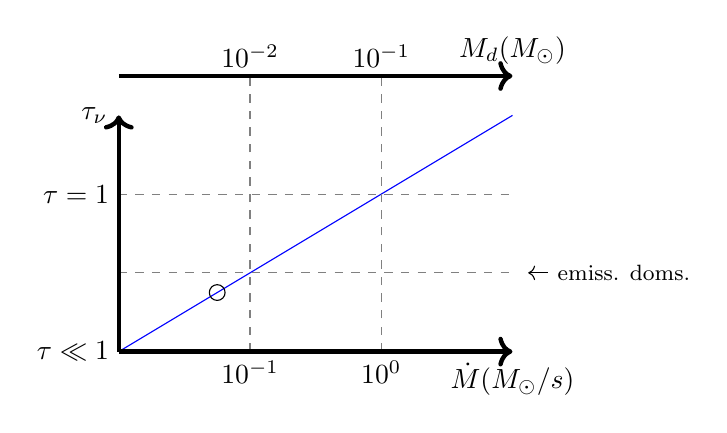
\begin{tikzpicture}
      \coordinate (origin) at (0,0);

      \draw[blue] (origin) -- (5,3);

      \node[left] (tau1) at (0,2) {$\tau=1$};
      \draw[dashed,gray] (tau1) -- ++(5.5,0);

      \node[below] (m1) at (10./3.,0) {$10^0$};
      \draw[dashed,gray] (m1) -- ++(0,3.75)
      node[above] {\color{black}$10^{-1}$};
      
      \coordinate(tau2) at (0,1);
      \draw[dashed,gray] (tau2) -- ++(5,0);

      \node[below](m2) at (5./3.,0) {$10^{-1}$};
      \draw[dashed, gray] (m2) -- ++(0, 3.75)
      node[above] {\color{black}$10^{-2}$};

      \node[left] at (origin) {$\tau\ll 1$};
      \draw[ultra thick, black,->] (origin)
      -- ++(5, 0) node[below] {$\dot{M} (M_\odot/s)$};
      \draw[ultra thick, black, ->] (origin)
      -- ++(0, 3) node[left] {$\tau_\nu$};
      \draw[ultra thick, black, ->] (0,3.5)
      -- ++(5,0) node[above] {$M_d (M_\odot)$};

      \draw[<-] (5.2,1) -- ++(0.25,0) node[right,align=left]
      {\footnotesize emiss. doms.};

      \draw (5./4.,3./4.) circle (0.1);
    \end{tikzpicture}
    }
\end{frame}

\begin{frame}
  \frametitle{Stationary Disk, No Ye equilibrium!}
  \setlength{\unitlength}{1cm}
  \begin{picture}(12,8)
    \visible<1>{
      \put(2, 0.5){
        \includegraphics[height=0.9\textheight]{collapsar/ye_statistics}
      }
    }
    \visible<2->{
      \put(0,1) {
        \includegraphics[width=0.5\textwidth]{collapsar/ye_statistics}
      }
      \put(6,4) {
        \includegraphics[width=0.5\textwidth]{collapsar/rho_Ye_snap_t5000}
      }
      \put(5,0.0) {
        \includegraphics[width=0.6\textwidth]{collapsar/selected_traces_lattitude_cut}
      }
      \put(0,0){
        {\footnotesize Miller et al., ApJ \textbf{902}, 66 (2020)}
      }
    }
  \end{picture}
\end{frame}

\begin{frame}
  \frametitle{Turbulence and $Y_e$}
  \resizebox{12cm}{!}{
    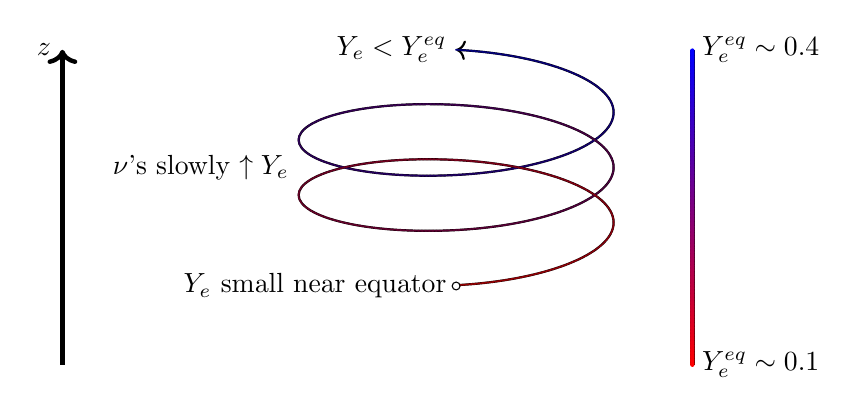
\begin{tikzpicture}
      \coordinate(origin) at (-2,0);

      \draw[ultra thick, black, ->] (origin) -- ++ (0, 4)
      node[left] {$z$};

      \draw[ultra thick,colormorph={0.8pt}{red}{blue}] (6,0) -- ++(0,4);
      \node[right] at (6,0) {$Y_e^{eq}\sim 0.1$};
      \node[right] at (6,4) {$Y_e^{eq}\sim 0.4$};

      \draw[thick,
      decoration={aspect=0.31,segment length=7mm,amplitude=2cm, coil},
      colormorph={0.4pt}{deepblue}{deepred},
      decorate,arrows={<[bend]-}] (3,4) -- (3,1);
      \node[draw,fill=white,circle,inner sep=1pt] at (3,1) {};
      \node[left] at (3,1) {$Y_e$ small near equator};
      \node[left] at (1.,2.5) {$\nu$'s slowly $\uparrow Y_e$};
      \node[left] at (3,4) {$Y_e < Y_e^{eq}$};
    \end{tikzpicture}
  }
\end{frame}

\begin{frame}
  \frametitle{$Y_e$ is set by the balance of Turbulence and
    Neutrinos!}
  \begin{center}
    \includegraphics[width=0.9\textwidth]{collapsar/ye_time_scales_t5000}
  \end{center}
  {\footnotesize Miller et al., ApJ \textbf{902}, 66 (2020)}
\end{frame}

\begin{frame}
  \frametitle{$Y_e$ is set by the balance of Turbulence and
    Neutrinos!}
  \begin{displaymath}
      Y_{\rm e}(z/H) = \braket{\text{min}(Y_{\rm e})}_{\text{trc}}
      + \braket{\frac{d Y_{\rm e}}{dt}}_{t,\text{trc}} \paren{H\braket{\frac{dz}{dt}}_{t,\text{trc}}^{-1}}\paren{\frac{z}{H} - \braket{\text{min}(z/H)}_{\text{trc}}}
    \end{displaymath}
    \begin{columns}
      \begin{column}{6cm}
        \includegraphics[width=\columnwidth]{collapsar/vertical-structure-params}
      \end{column}
      \begin{column}{6cm}
        \includegraphics[width=\columnwidth]{collapsar/model-vs-vertical-structure}
      \end{column}
    \end{columns}
    {\footnotesize Miller et al., ApJ \textbf{902}, 66 (2020)}
  \end{frame}

\begin{frame}
  \frametitle{Future}
  \begin{itemize}
  \item Large optical depths, such as inside a neutron star present issues for Monte Carlo
  \item Need a method that can span the range of optical depths and solve the full transport equation
  \end{itemize}
  \begin{center}
    \includegraphics[width=\textwidth]{mocmc-diagram};
  \end{center}
\end{frame}

\begin{frame}
  \frametitle{Conclusions}
  \begin{columns}
    \begin{column}{7cm}
      \begin{itemize}
      \item Need GRRMHD and neutrino transport!
      \item NS Mergers:
        \begin{itemize}
        \item Likely source of heavy elements in our
          universe
        \item Disks can produce blue component of kilonova
        \end{itemize}
      \item Large diversity in outflows and disk physics
        \begin{itemize}
        \item Angular structure in the outflow is generic.
        \item Set by balance between MHD turbulence and neutrino physics
        \end{itemize}
      \item Stay tuned for more
      \end{itemize}
    \end{column}
    \begin{column}{5cm}
      \includegraphics[width=\columnwidth,clip,trim={150 0 150 0}]{3d_render}
    \end{column}
  \end{columns}
\end{frame}

\backupbegin

\begin{frame}
  \frametitle{Accretion Rates}
  \begin{center}
    \includegraphics[width=0.9\textwidth]{mdot_edd}
  \end{center}
\end{frame}

\begin{frame}
  \frametitle{Accretion Rates}
  \begin{center}
    \includegraphics[width=0.9\textwidth]{mdot_edd_nu}
  \end{center}
\end{frame}

% \begin{frame}
%   \frametitle{A Growing Suite of Models}
%   \begin{columns}
%     \begin{column}{5cm}
%       \begin{center}
%         \includegraphics[width=\columnwidth]{disks_run_MMa_3d_scatter}
%       \end{center}
%     \end{column}
%     \begin{column}{7cm}
%       \resizebox{\columnwidth}{!}{
%         \begin{tikzpicture}
%           \coordinate (origin) at (0,0);
%           \pgfmathsetmacro{\pi}{3.14159}
%           \pgfmathsetmacro{\dbx}{0.5}
%           \pgfmathsetmacro{\dby}{0.05}
%           \pgfmathsetmacro{\dex}{2.}
%           \pgfmathsetmacro{\dey}{0.25}
%           \pgfmathsetmacro{\dcc}{2.1}
%           \pgfmathsetmacro{\tcx}{5.0}
%           \pgfmathsetmacro{\rstar}{5}
%           \pgfmathsetmacro{\wstar}{0.25}
%           \pgfmathsetmacro{\wjet}{0.75}
%           \pgfmathsetmacro{\tangle}{{45}}
%           \pgfmathsetmacro{\tsx}{{(\rstar+\wstar)*cos(\tangle)}}
%           \pgfmathsetmacro{\tsy}{{(\rstar+\wstar)*sin(\tangle)}}
% 
%           \pgfmathsetmacro{\cangle}{15}
%           \pgfmathsetmacro{\cx}{(\rstar-\wstar)*cos(\cangle)}
%           \pgfmathsetmacro{\cy}{(\rstar-\wstar)*sin(\cangle)}
%           % \pgfmathsetmacro{\cend}{\dex + 0.1}
%           \pgfmathsetmacro{\cend}{\dbx + 0.1}
% 
%           \newcommand{\msize}{\huge}
% 
%           % star
%           \fill [color=red] (origin) circle (\rstar+\wstar);
%           \fill [color=white] (origin) circle (\rstar-\wstar);
% 
%           % circularization
%           \fill[color=red,
%           left color=orange,
%           middle color=orange,
%           right color=red]
%           (\cx,\cy) to [bend left=10] (\cend,0)
%           to [bend left=10] (\cx,-\cy)
%           to [bend right=20] cycle;
%           
%           \draw[orange,ultra thick]
%           (\cx,\cy) to [bend left=10] (\cend, 0)
%           to [bend left=10] (\cx,-\cy);
% 
%           \fill[color=red,
%           right color=orange,
%           middle color=orange,
%           left color=red]
%           (-\cx,\cy) to [bend right=10] (-\cend,0)
%           to [bend right=10] (-\cx,-\cy)
%           to [bend left=20] cycle;
%           
%           \draw[orange,ultra thick]
%           (-\cx,\cy) to [bend right=10] (-\cend, 0)
%           to [bend right=10] (-\cx,-\cy);
% 
%           % \foreach \i in {-1,1}
%           % {
%           %   % disk
%           %   \fill[color=orange]
%           %   (\i*\dbx,\dby) -- (\i*\dex,\dey)
%           %   .. controls (\i*\dcc,0) .. (\i*\dex,-\dey)
%           %   -- (\i*\dbx,-\dby) -- cycle;
%           % }
%           
%           % jet
%           \fill[color=blue] (origin) -- (-\wjet,1.25*\rstar) -- ++(2*\wjet,0) -- cycle;
% 
%           % bh
%           \shade[ball color=black] (origin) circle (0.25);
% 
%           % wind
%           \draw[deepgreen,ultra thick, ->]
%           ({0.5*(\dbx + \dex)},\dey) -- ++(2,2);
%           \draw ({0.5*(\dbx + \dex) + 1},{(\dey+1)})
%           node[above,align=center,rotate=45]
%           {\color{deepgreen}\msize wind};
%           \draw[deepgreen,ultra thick, ->]
%           ({-0.5*(\dbx + \dex)},\dey) -- ++(-2,2);
%           \draw ({-(0.5*(\dbx + \dex) + 1)},{(\dey+1)})
%           node[above,align=center,rotate=-45]
%           {\color{deepgreen}\msize wind};          
% 
%           % text
%           \draw[<-,orange, ultra thick] (\dex-0.1,-\dey-0.1)
%           -- ++(3,-5) -- ++(1,0)
%           node[right,align=left]
%           {\msize \color{orange}Disk};
%           
%           \draw[<-,black, ultra thick] (-0.25,-0.25)
%           -- ++(-3,-5) -- ++(-1,0)
%           node[left,align=right]
%           {\msize \color{black}Black Hole\\ \msize $\sim 3 M_{\odot}$};
%           
%           \draw[<-,red,ultra thick] (\tsx,\tsy)
%           -- ++(1,1) -- ++(1,0)
%           node[right,align=left]
%           {\msize \color{red} Stellar\\ \msize envelope};
% 
%           \draw[<-,blue,ultra thick] (0, 1.25*\rstar) -- ++(0,1)
%           node[above,align=center] {\msize \color{blue} Jet};
% 
%           \draw[<-,black,ultra thick]
%           ({0.5*(\dex+\rstar)},0) -- ++(2,0) node[right,align=left]
%           {\msize Circularizing\\ \msize material};
%           
%           \let\msize\undefined
%         \end{tikzpicture}
%       }
%     \end{column}
%   \end{columns}
% \end{frame}

% \begin{frame}
%   \frametitle{A Growing Suite of Models}
%   \begin{columns}
%     \begin{column}{4cm}
%       \begin{center}
%         \includegraphics[width=\columnwidth]{disks_run_MMa_3d_scatter}
%       \end{center}
%     \end{column}
%     \begin{column}{8cm}
%       \begin{center}
%         \includegraphics[width=\columnwidth]{disks_run_thermo_params}
%       \end{center}
%     \end{column}
%   \end{columns}
%   \begin{itemize}
%   \item Soon to be many more.
%   \item $\gtrapprox 50$ by the end of the DR
%   \end{itemize}
% \end{frame}

\begin{frame}
  \frametitle{What is a Collapsar?}
  \begin{columns}
    \begin{column}{5cm}
      \begin{itemize}
      \item Accretion times $t\sim 10s$
      \item $\dot{M}$ between
        \begin{itemize}
        \item $10^{-4} M_\odot/s$
        \item $10^{-1} M_\odot/s$ 
        \end{itemize}
      \item $\rho \sim 10^{10}$ g$/$cm$^3$
      \end{itemize}
      \resizebox{\columnwidth}{!}{
        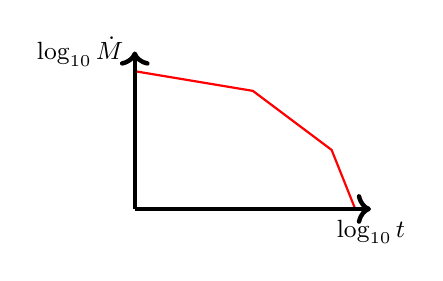
\begin{tikzpicture}
          \draw[thick,red]
          (0,1.75) -- (1.5,1.5) -- (2.5,0.75) -- (2.8,0);

          \coordinate (origin) at (0,0);
          \draw[ultra thick,->]
          (origin) -- ++(3,0)
          node[below] {\small $\log_{10}t$};
          \draw[ultra thick,->]
          (origin) -- ++(0,2)
          node[left] {\small $\log_{10}\dot{M}$};
        \end{tikzpicture}
      }
      \begin{tiny}
        Siegel, Barnes, Metzger. Nature \textbf{241} (2019)
      \end{tiny}
    \end{column}
    \begin{column}{7cm}
      \resizebox{\columnwidth}{!}{
        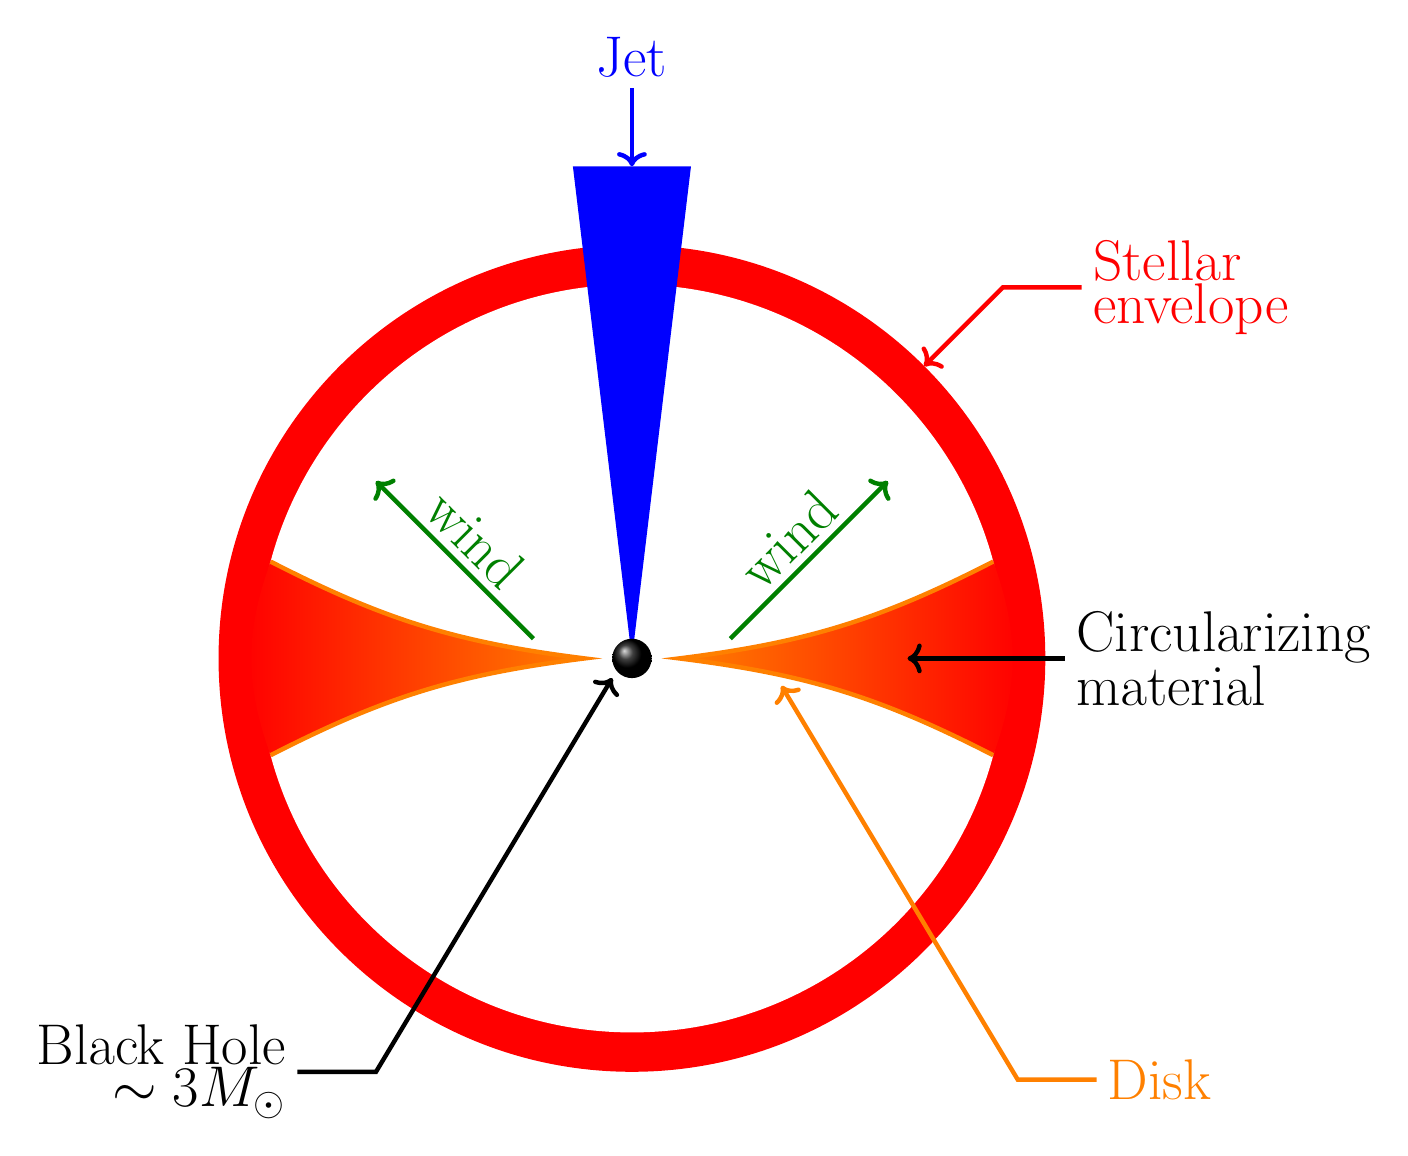
\begin{tikzpicture}
          \coordinate (origin) at (0,0);
          \pgfmathsetmacro{\pi}{3.14159}
          \pgfmathsetmacro{\dbx}{0.5}
          \pgfmathsetmacro{\dby}{0.05}
          \pgfmathsetmacro{\dex}{2.}
          \pgfmathsetmacro{\dey}{0.25}
          \pgfmathsetmacro{\dcc}{2.1}
          \pgfmathsetmacro{\tcx}{5.0}
          \pgfmathsetmacro{\rstar}{5}
          \pgfmathsetmacro{\wstar}{0.25}
          \pgfmathsetmacro{\wjet}{0.75}
          \pgfmathsetmacro{\tangle}{{45}}
          \pgfmathsetmacro{\tsx}{{(\rstar+\wstar)*cos(\tangle)}}
          \pgfmathsetmacro{\tsy}{{(\rstar+\wstar)*sin(\tangle)}}

          \pgfmathsetmacro{\cangle}{15}
          \pgfmathsetmacro{\cx}{(\rstar-\wstar)*cos(\cangle)}
          \pgfmathsetmacro{\cy}{(\rstar-\wstar)*sin(\cangle)}
          % \pgfmathsetmacro{\cend}{\dex + 0.1}
          \pgfmathsetmacro{\cend}{\dbx + 0.1}

          \newcommand{\msize}{\huge}

          % star
          \fill [color=red] (origin) circle (\rstar+\wstar);
          \fill [color=white] (origin) circle (\rstar-\wstar);

          % circularization
          \fill[color=red,
          left color=orange,
          middle color=orange,
          right color=red]
          (\cx,\cy) to [bend left=10] (\cend,0)
          to [bend left=10] (\cx,-\cy)
          to [bend right=20] cycle;
          
          \draw[orange,ultra thick]
          (\cx,\cy) to [bend left=10] (\cend, 0)
          to [bend left=10] (\cx,-\cy);

          \fill[color=red,
          right color=orange,
          middle color=orange,
          left color=red]
          (-\cx,\cy) to [bend right=10] (-\cend,0)
          to [bend right=10] (-\cx,-\cy)
          to [bend left=20] cycle;
          
          \draw[orange,ultra thick]
          (-\cx,\cy) to [bend right=10] (-\cend, 0)
          to [bend right=10] (-\cx,-\cy);

          % \foreach \i in {-1,1}
          % {
          %   % disk
          %   \fill[color=orange]
          %   (\i*\dbx,\dby) -- (\i*\dex,\dey)
          %   .. controls (\i*\dcc,0) .. (\i*\dex,-\dey)
          %   -- (\i*\dbx,-\dby) -- cycle;
          % }
          
          % jet
          \fill[color=blue] (origin) -- (-\wjet,1.25*\rstar) -- ++(2*\wjet,0) -- cycle;

          % bh
          \shade[ball color=black] (origin) circle (0.25);

          % wind
          \draw[deepgreen,ultra thick, ->]
          ({0.5*(\dbx + \dex)},\dey) -- ++(2,2);
          \draw ({0.5*(\dbx + \dex) + 1},{(\dey+1)})
          node[above,align=center,rotate=45]
          {\color{deepgreen}\msize wind};
          \draw[deepgreen,ultra thick, ->]
          ({-0.5*(\dbx + \dex)},\dey) -- ++(-2,2);
          \draw ({-(0.5*(\dbx + \dex) + 1)},{(\dey+1)})
          node[above,align=center,rotate=-45]
          {\color{deepgreen}\msize wind};          

          % text
          \draw[<-,orange, ultra thick] (\dex-0.1,-\dey-0.1)
          -- ++(3,-5) -- ++(1,0)
          node[right,align=left]
          {\msize \color{orange}Disk};
          
          \draw[<-,black, ultra thick] (-0.25,-0.25)
          -- ++(-3,-5) -- ++(-1,0)
          node[left,align=right]
          {\msize \color{black}Black Hole\\ \msize $\sim 3 M_{\odot}$};
          
          \draw[<-,red,ultra thick] (\tsx,\tsy)
          -- ++(1,1) -- ++(1,0)
          node[right,align=left]
          {\msize \color{red} Stellar\\ \msize envelope};

          \draw[<-,blue,ultra thick] (0, 1.25*\rstar) -- ++(0,1)
          node[above,align=center] {\msize \color{blue} Jet};

          \draw[<-,black,ultra thick]
          ({0.5*(\dex+\rstar)},0) -- ++(2,0) node[right,align=left]
          {\msize Circularizing\\ \msize material};
          
          \let\msize\undefined
        \end{tikzpicture}
      }
    \end{column}
  \end{columns}
\end{frame}

\backupend

\end{document}